\documentclass[11pt,a4paper]{article}

% ── Packages ──────────────────────────────────────────────────────────────────
\usepackage[utf8]{inputenc}
\usepackage[T1]{fontenc}
\usepackage{amsmath,amssymb,amsthm}
\usepackage{booktabs}
\usepackage{graphicx}
\usepackage{hyperref}
\usepackage[margin=2.5cm]{geometry}
\usepackage{algorithm}
\usepackage{algpseudocode}
\usepackage{caption}
\usepackage{subcaption}
\usepackage{enumitem}
\usepackage{xcolor}
\usepackage{listings}
\usepackage{array}

\hypersetup{
  colorlinks=true,
  linkcolor=blue!70!black,
  citecolor=green!50!black,
  urlcolor=blue!60!black,
}

\lstset{
  basicstyle=\ttfamily\small,
  breaklines=true,
  frame=single,
  backgroundcolor=\color{gray!5},
  keywordstyle=\color{blue!70!black},
  commentstyle=\color{green!50!black},
  stringstyle=\color{red!60!black},
}

\newcommand{\gen}[1]{\langle #1 \rangle}
\newcommand{\pres}[2]{\langle #1 \mid #2 \rangle}
\newcommand{\inv}[1]{#1^{-1}}

% ── Title ─────────────────────────────────────────────────────────────────────
\title{Reproducing Results on the Andrews--Curtis Conjecture:\\
  Classical Search and PPO}
\author{AC-Solver Project}
\date{April 2026}

\begin{document}
\maketitle

\begin{abstract}
This document provides a self-contained account of our reproduction experiments
on the Andrews--Curtis conjecture using the Miller--Schupp dataset (1190
balanced presentations).  We describe (1)~the classical search algorithms
(greedy and breadth-first) including pseudocode, exact reproduction commands,
and results; (2)~a Proximal Policy Optimisation (PPO) agent trained for $10^8$
environment steps, its architecture, hyperparameters, training dynamics, and
evaluation; and (3)~a comparative analysis showing that the PPO agent learns
genuine but shallow problem structure, solving $2.7\%$ of instances at best
versus $46.6\%$ for greedy search.  All commands needed to reproduce every
result are collected in Appendix~\ref{sec:commands}.
\end{abstract}

\tableofcontents
\newpage

% ══════════════════════════════════════════════════════════════════════════════
\section{Introduction}\label{sec:intro}
% ══════════════════════════════════════════════════════════════════════════════

\subsection{The Andrews--Curtis Conjecture}

The \emph{Andrews--Curtis conjecture} (1965) asserts that every balanced
presentation of the trivial group can be reduced to the standard trivial
presentation $\pres{x,y}{x,y}$ using a finite sequence of \emph{AC moves}:
Nielsen transformations on relators and conjugation by generators.  Despite
extensive computational and theoretical effort, the conjecture remains open.

Computationally, the problem reduces to a \emph{graph search}: each node is a
balanced presentation $\pres{x,y}{r_0, r_1}$, each edge is one of 12~AC moves,
and the goal is to reach a trivial node (total relator length~$= 2$).

\subsection{The Miller--Schupp Dataset}

We use the Miller--Schupp family of presentations, parameterised by an integer
$n \ge 1$ and a balanced word $w$ over $\{x, \inv{x}, y, \inv{y}\}$:
\[
  \mathrm{MS}(n, w) \;=\; \pres{x, y}{\inv{x}\, y^n\, x\, y^{-(n+1)},\;\; \inv{x}\, w}.
\]
With $n \in \{1, \ldots, 7\}$ and $|w| \in \{1, \ldots, 7\}$, after removing
cyclic permutations and applying free/cyclic reduction, the dataset contains
\textbf{1190~presentations}.  These are stored in
\texttt{ac\_solver/search/miller\_schupp/data/all\_presentations.txt}, one
per line.

\subsection{Presentation Encoding}

Each presentation is encoded as a NumPy \texttt{int8} array of length
$2 \times \texttt{max\_relator\_length}$.  The first half stores~$r_0$ and the
second half stores~$r_1$, both right-padded with zeros:
\begin{center}
\begin{tabular}{cl}
  \toprule
  \textbf{Value} & \textbf{Meaning} \\
  \midrule
  $+1$ & generator $x$ \\
  $-1$ & generator $\inv{x}$ \\
  $+2$ & generator $y$ \\
  $-2$ & generator $\inv{y}$ \\
  $\phantom{+}0$ & padding (unused position) \\
  \bottomrule
\end{tabular}
\end{center}
For the Miller--Schupp dataset, $\texttt{max\_relator\_length} = 36$
(derived from $\max_n(4n+2)$ for $n \le 7$), giving observation vectors of
dimension~72.

\subsection{Success Criterion}

A presentation is \emph{solved} (trivialised) when the sum of both relators'
non-zero lengths equals~2, i.e.\ each relator is a single generator or its
inverse.  For example, $\pres{x,y}{x, \inv{y}}$ is trivial.

% ══════════════════════════════════════════════════════════════════════════════
\section{The 12 AC Moves}\label{sec:moves}
% ══════════════════════════════════════════════════════════════════════════════

At each state, there are 12 possible actions: 4~concatenations and
8~conjugations.  After every move, \emph{free reduction} is applied
automatically (cancelling adjacent inverse pairs such as $x \cdot \inv{x}$).
If the resulting relator would exceed \texttt{max\_relator\_length}, the move is
rejected and the state is returned unchanged (a ``no-op'').

\begin{table}[h]
\centering
\caption{The 12 AC moves.  Here $x_1 = x$, $x_2 = y$.}
\label{tab:moves}
\small
\begin{tabular}{clll}
  \toprule
  \textbf{ID} & \textbf{Type} & \textbf{Operation} & \textbf{Description} \\
  \midrule
  0  & Concat & $r_1 \leftarrow r_1 \cdot r_0$               & Append $r_0$ to $r_1$ \\
  1  & Concat & $r_0 \leftarrow r_0 \cdot \inv{r_1}$         & Append $\inv{r_1}$ to $r_0$ \\
  2  & Concat & $r_1 \leftarrow r_1 \cdot \inv{r_0}$         & Append $\inv{r_0}$ to $r_1$ \\
  3  & Concat & $r_0 \leftarrow r_0 \cdot r_1$               & Append $r_1$ to $r_0$ \\
  \midrule
  4  & Conj   & $r_1 \leftarrow \inv{x} \cdot r_1 \cdot x$   & Conjugate $r_1$ by $\inv{x}$ \\
  5  & Conj   & $r_0 \leftarrow \inv{y} \cdot r_0 \cdot y$   & Conjugate $r_0$ by $\inv{y}$ \\
  6  & Conj   & $r_1 \leftarrow \inv{y} \cdot r_1 \cdot y$   & Conjugate $r_1$ by $\inv{y}$ \\
  7  & Conj   & $r_0 \leftarrow x \cdot r_0 \cdot \inv{x}$   & Conjugate $r_0$ by $x$ \\
  8  & Conj   & $r_1 \leftarrow x \cdot r_1 \cdot \inv{x}$   & Conjugate $r_1$ by $x$ \\
  9  & Conj   & $r_0 \leftarrow y \cdot r_0 \cdot \inv{y}$   & Conjugate $r_0$ by $y$ \\
  10 & Conj   & $r_1 \leftarrow y \cdot r_1 \cdot \inv{y}$   & Conjugate $r_1$ by $y$ \\
  11 & Conj   & $r_0 \leftarrow \inv{x} \cdot r_0 \cdot x$   & Conjugate $r_0$ by $\inv{x}$ \\
  \bottomrule
\end{tabular}
\end{table}

\paragraph{Free Reduction.}
After every move, adjacent inverse pairs are cancelled iteratively.  For
example, if a concatenation produces $\ldots x \cdot \inv{x} \ldots$, the pair
is removed.  This is applied until no more cancellations are possible.

\paragraph{Move Rejection.}
If the resulting relator would have length $> 36$ (after free reduction), the
move returns the original state unchanged.  This is a significant source of
``no-op'' steps: approximately $69\%$ of actions during PPO training produce no
state change.

% ══════════════════════════════════════════════════════════════════════════════
\section{Classical Search Algorithms}\label{sec:classical}
% ══════════════════════════════════════════════════════════════════════════════

Both algorithms explore the same graph of balanced presentations.  They differ
only in the order states are expanded: greedy uses a priority queue ordered by
total relator length; BFS uses a FIFO queue ordered by insertion time (depth).

\subsection{Greedy Search}\label{sec:greedy}

\paragraph{Core idea.}
Always expand the state with the \emph{shortest total presentation length}
first, using a min-heap.  This is a heuristic: it assumes shorter presentations
are closer to the trivial state.

\begin{algorithm}[H]
\caption{Greedy Search for AC Trivialisation}
\label{alg:greedy}
\begin{algorithmic}[1]
\Require Presentation $P$, max nodes $N$
\Ensure \textsc{True}/\textsc{False}, path, visited count
\State $L \gets \textsc{MaxRelatorLength}(P)$
\State $\ell_0, \ell_1 \gets \textsc{WordLengths}(P)$
\State $\textit{visited} \gets \{P\}$
\State $\textit{heap} \gets [(\ell_0 + \ell_1,\; 0,\; P,\; (\ell_0, \ell_1),\; [(-1, \ell_0+\ell_1)])]$
  \Comment{priority, depth, state, lengths, path}
\While{$\textit{heap} \neq \emptyset$ \textbf{and} $|\textit{visited}| < N$}
  \State $(\_, d, S, w, \textit{path}) \gets \textsc{HeapPop}(\textit{heap})$
  \For{$a \in \{0, 1, \ldots, 11\}$}
    \State $S', w' \gets \textsc{ACMove}(a, S, L, w)$
    \State $\ell' \gets w'_0 + w'_1$
    \If{$\ell' = 2$}
      \State \Return \textsc{True}, $\textit{path} \mathbin\Vert [(a, \ell')]$, $|\textit{visited}|$
    \EndIf
    \If{$S' \notin \textit{visited}$}
      \State $\textit{visited} \gets \textit{visited} \cup \{S'\}$
      \State $\textsc{HeapPush}(\textit{heap},\; (\ell',\; d+1,\; S',\; w',\; \textit{path} \mathbin\Vert [(a, \ell')]))$
    \EndIf
  \EndFor
\EndWhile
\State \Return \textsc{False}, $\textit{path}$, $|\textit{visited}|$
\end{algorithmic}
\end{algorithm}

\paragraph{Tie-breaking.}
When two states share the same total length, the heap breaks ties by
(i)~path length (prefer fewer moves from start), then (ii)~lexicographic
comparison of the state tuple.

\paragraph{Properties.}
\begin{itemize}[nosep]
  \item \textbf{No shortest-path guarantee.}  Greedy may find a solution via a
    longer path because it chases locally short states.
  \item \textbf{Typically faster.}  By focusing on short states, it often
    explores fewer nodes than BFS.
  \item \textbf{Per-step cost:} $O(\log n)$ for heap operations.
\end{itemize}

\paragraph{Source code.}
\texttt{ac\_solver/search/greedy.py}, function \texttt{greedy\_search()}.

% ──────────────────────────────────────────────────────────────────────────────
\subsection{Breadth-First Search (BFS)}\label{sec:bfs}

\paragraph{Core idea.}
Expand states strictly level by level---all states reachable in $d$~moves
before any state at depth $d+1$---using a FIFO queue.  Because every AC move
has unit cost, BFS \emph{guarantees finding the shortest path} (fewest moves).

\begin{algorithm}[H]
\caption{Breadth-First Search for AC Trivialisation}
\label{alg:bfs}
\begin{algorithmic}[1]
\Require Presentation $P$, max nodes $N$
\Ensure \textsc{True}/\textsc{False}, path, visited count
\State $L \gets \textsc{MaxRelatorLength}(P)$
\State $\textit{visited} \gets \{P\}$
\State $\textit{queue} \gets \textsc{Deque}([(P,\; [(-1, \textsc{TotalLength}(P))])])$
\While{$\textit{queue} \neq \emptyset$ \textbf{and} $|\textit{visited}| < N$}
  \State $(S, \textit{path}) \gets \textsc{PopLeft}(\textit{queue})$
  \State $w \gets \textsc{WordLengths}(S)$
    \Comment{Recomputed from current state}
  \For{$a \in \{0, 1, \ldots, 11\}$}
    \State $S', w' \gets \textsc{ACMove}(a, S, L, w)$
    \State $\ell' \gets w'_0 + w'_1$
    \If{$\ell' = 2$}
      \State \Return \textsc{True}, $\textit{path} \mathbin\Vert [(a, \ell')]$, $|\textit{visited}|$
    \EndIf
    \If{$S' \notin \textit{visited}$}
      \State $\textit{visited} \gets \textit{visited} \cup \{S'\}$
      \State $\textsc{Append}(\textit{queue},\; (S',\; \textit{path} \mathbin\Vert [(a, \ell')]))$
    \EndIf
  \EndFor
\EndWhile
\State \Return \textsc{False}, \textsc{None}, $|\textit{visited}|$
\end{algorithmic}
\end{algorithm}

\paragraph{Why BFS guarantees the shortest path.}
All states at depth~$d$ are expanded before any at depth $d+1$.  The first
time BFS reaches a trivial state, it must be via a minimum-length path---all
shorter paths have already been fully explored.

\paragraph{Properties.}
\begin{itemize}[nosep]
  \item \textbf{Shortest-path guarantee.}  The first solution found has the
    fewest AC moves of any solution within the node budget.
  \item \textbf{Typically slower.}  Exhaustive level-by-level expansion explores
    many more nodes than greedy.
  \item \textbf{Per-step cost:} $O(1)$ for deque append/popleft.
\end{itemize}

\paragraph{Source code.}
\texttt{ac\_solver/search/breadth\_first.py}, function \texttt{bfs()}.

% ──────────────────────────────────────────────────────────────────────────────
\subsection{Side-by-Side Comparison}

\begin{table}[h]
\centering
\caption{Greedy vs.\ BFS comparison.}
\label{tab:greedy-vs-bfs}
\begin{tabular}{lll}
  \toprule
  \textbf{Aspect} & \textbf{Greedy} & \textbf{BFS} \\
  \midrule
  Data structure     & Min-heap (priority queue)           & FIFO queue (deque) \\
  Expansion order    & Shortest total length first         & By depth (oldest first) \\
  Shortest path?     & No                                  & Yes (guaranteed) \\
  Typical speed      & Faster (fewer nodes explored)       & Slower (exhaustive per level) \\
  Per-step cost      & $O(\log n)$                         & $O(1)$ \\
  \bottomrule
\end{tabular}
\end{table}

% ──────────────────────────────────────────────────────────────────────────────
\subsection{Classical Search Results}\label{sec:classical-results}

Both algorithms were run on all 1190 Miller--Schupp presentations with a node
budget of $10^6$.

\begin{table}[h]
\centering
\caption{Classical search results (node budget = $10^6$).}
\label{tab:classical-results}
\begin{tabular}{lrrr}
  \toprule
  \textbf{Algorithm} & \textbf{Solved} & \textbf{Solve Rate} & \textbf{Paper Reference} \\
  \midrule
  Greedy  & 554 / 1190 & 46.6\% & 533 / 1190 (44.8\%) \\
  BFS     & 278 / 1190 & 23.4\% & 278 / 1190 (23.4\%) \\
  \bottomrule
\end{tabular}
\end{table}

Our BFS result matches the paper exactly.  Greedy search solves 21~more
instances than reported in the paper ($554$ vs.\ $533$); this small discrepancy
likely reflects minor implementation differences in tie-breaking or free
reduction.

\paragraph{How to reproduce.}
\begin{lstlisting}[language=bash]
# Greedy search on full dataset (1M node budget, 4 workers)
python -m ac_solver.search.miller_schupp.evaluate \
    --search-fn greedy --max-nodes 1000000 \
    --workers 4 --full --output results/greedy_1M.csv

# BFS on full dataset
python -m ac_solver.search.miller_schupp.evaluate \
    --search-fn bfs --max-nodes 1000000 \
    --workers 4 --full --output results/bfs_1M.csv
\end{lstlisting}

\paragraph{Results by difficulty.}
Figure~\ref{fig:classical-results} shows the solve rate broken down by the
Miller--Schupp parameters $n$ (relator complexity) and $|w|$ (word length), and
a heatmap of solve rate by $(n, |w|)$.

\begin{figure}[ht]
\centering
\begin{subfigure}[b]{0.48\textwidth}
  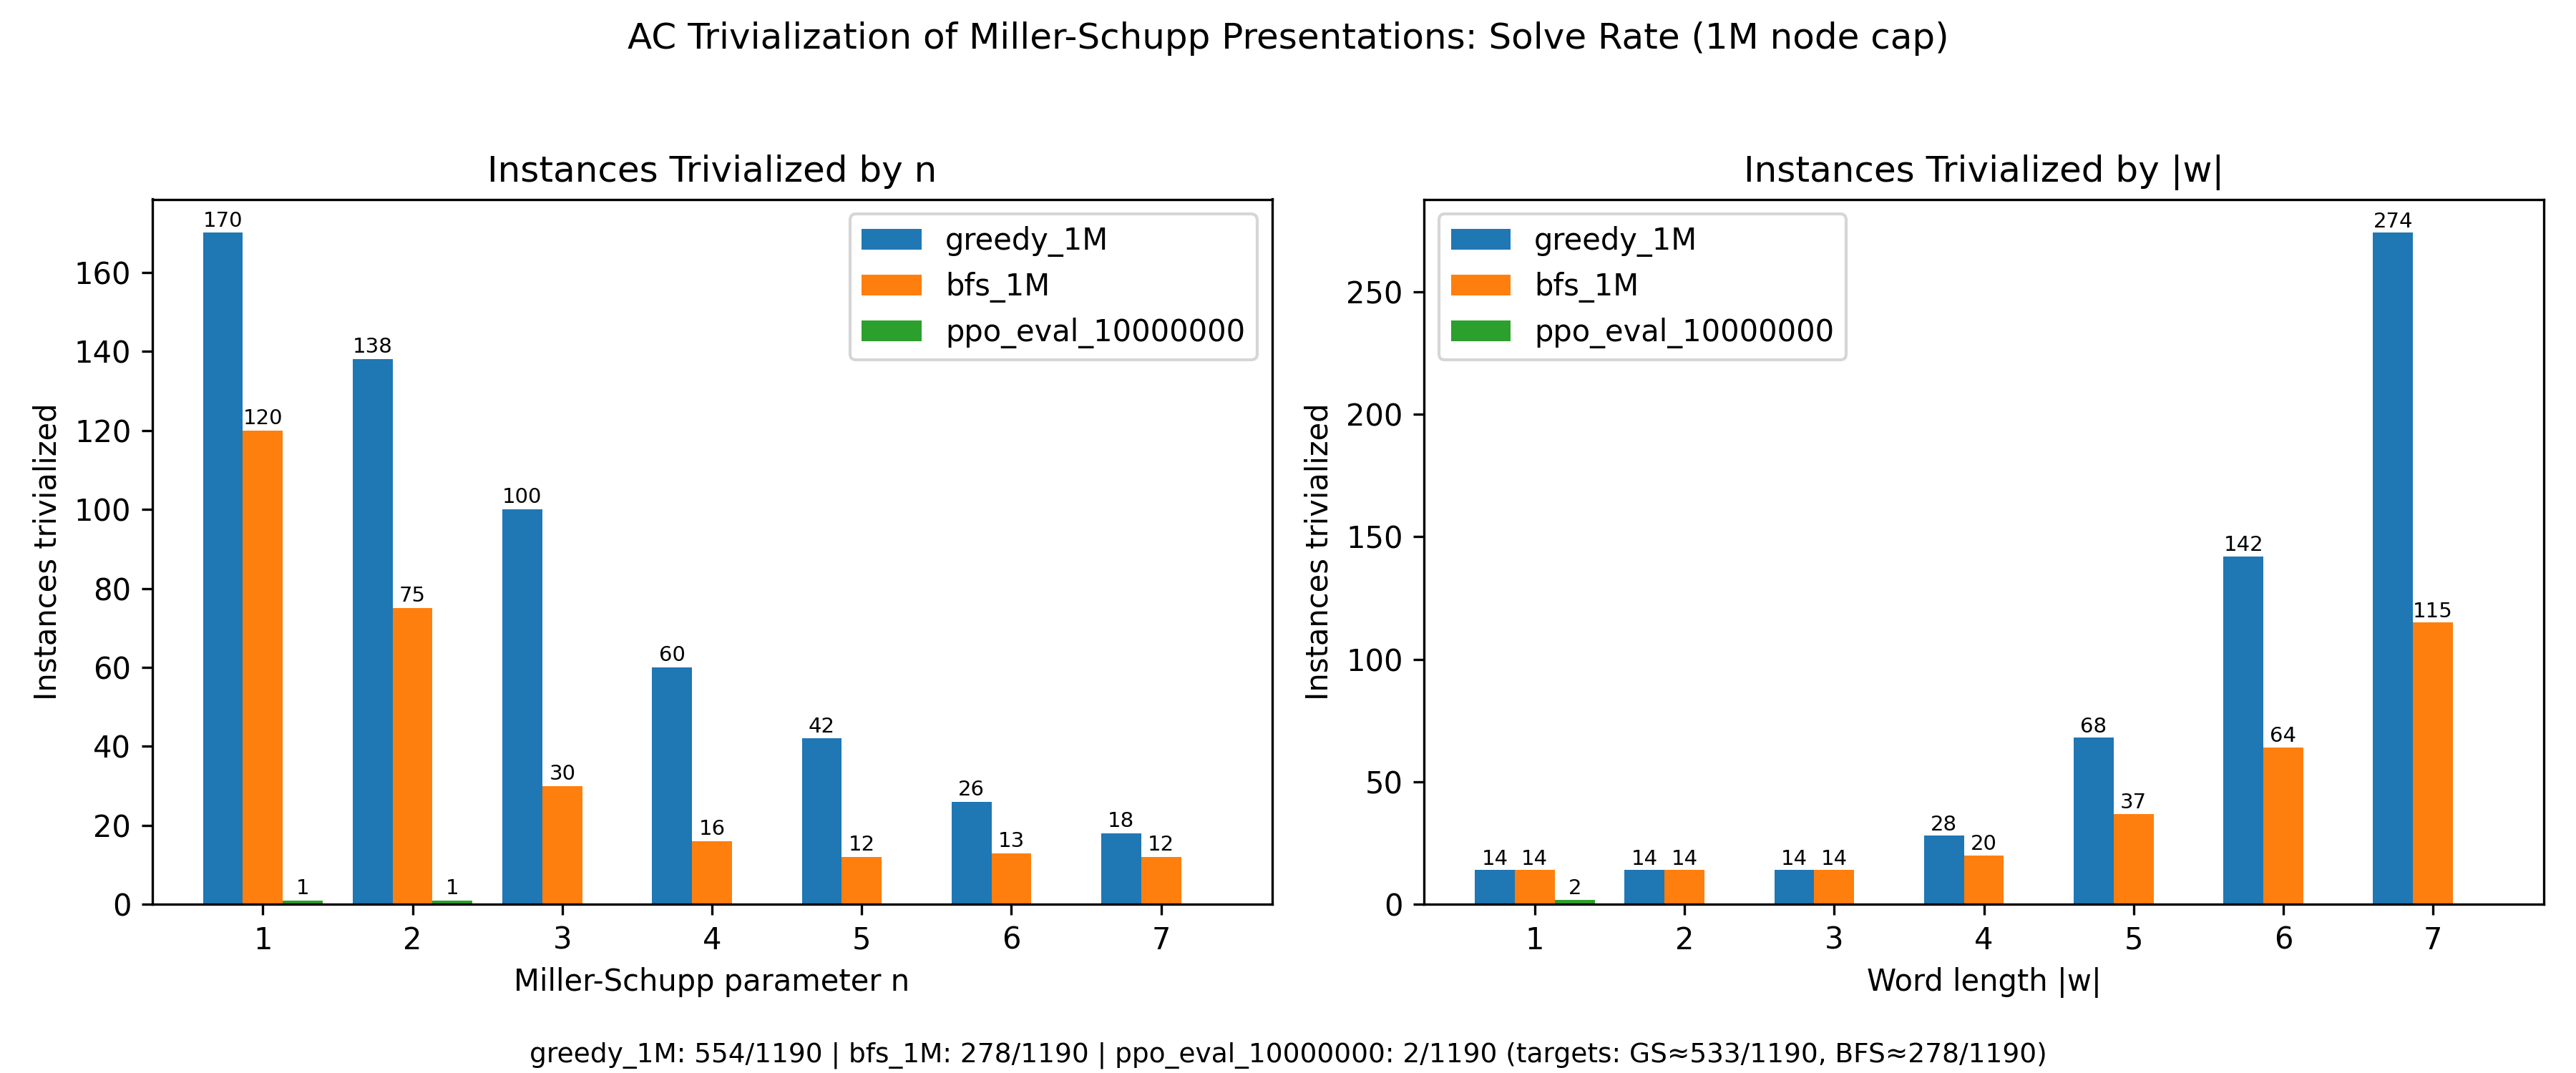
\includegraphics[width=\textwidth]{figures/ac_trivialization_solve_rate.png}
  \caption{Solve rate by $n$ and $|w|$.}
  \label{fig:solve-rate}
\end{subfigure}
\hfill
\begin{subfigure}[b]{0.48\textwidth}
  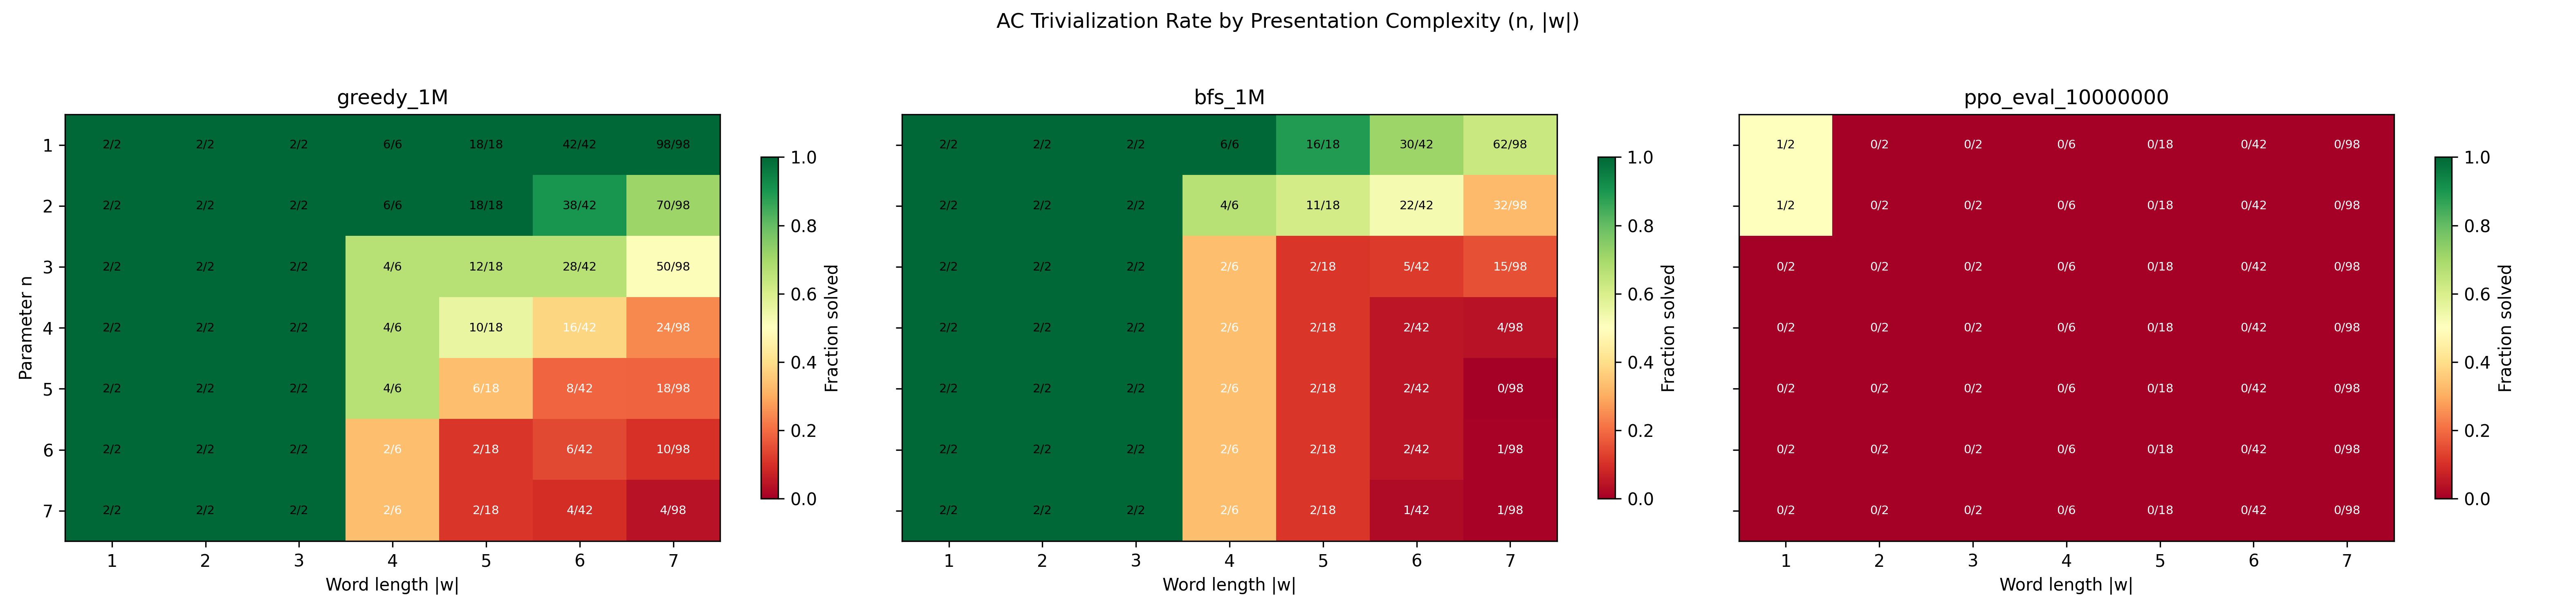
\includegraphics[width=\textwidth]{figures/ac_trivialization_heatmap_n_vs_w.png}
  \caption{Heatmap: solve rate by $(n, |w|)$.}
  \label{fig:heatmap}
\end{subfigure}
\caption{Classical search results on the Miller--Schupp dataset.}
\label{fig:classical-results}
\end{figure}

\begin{figure}[ht]
\centering
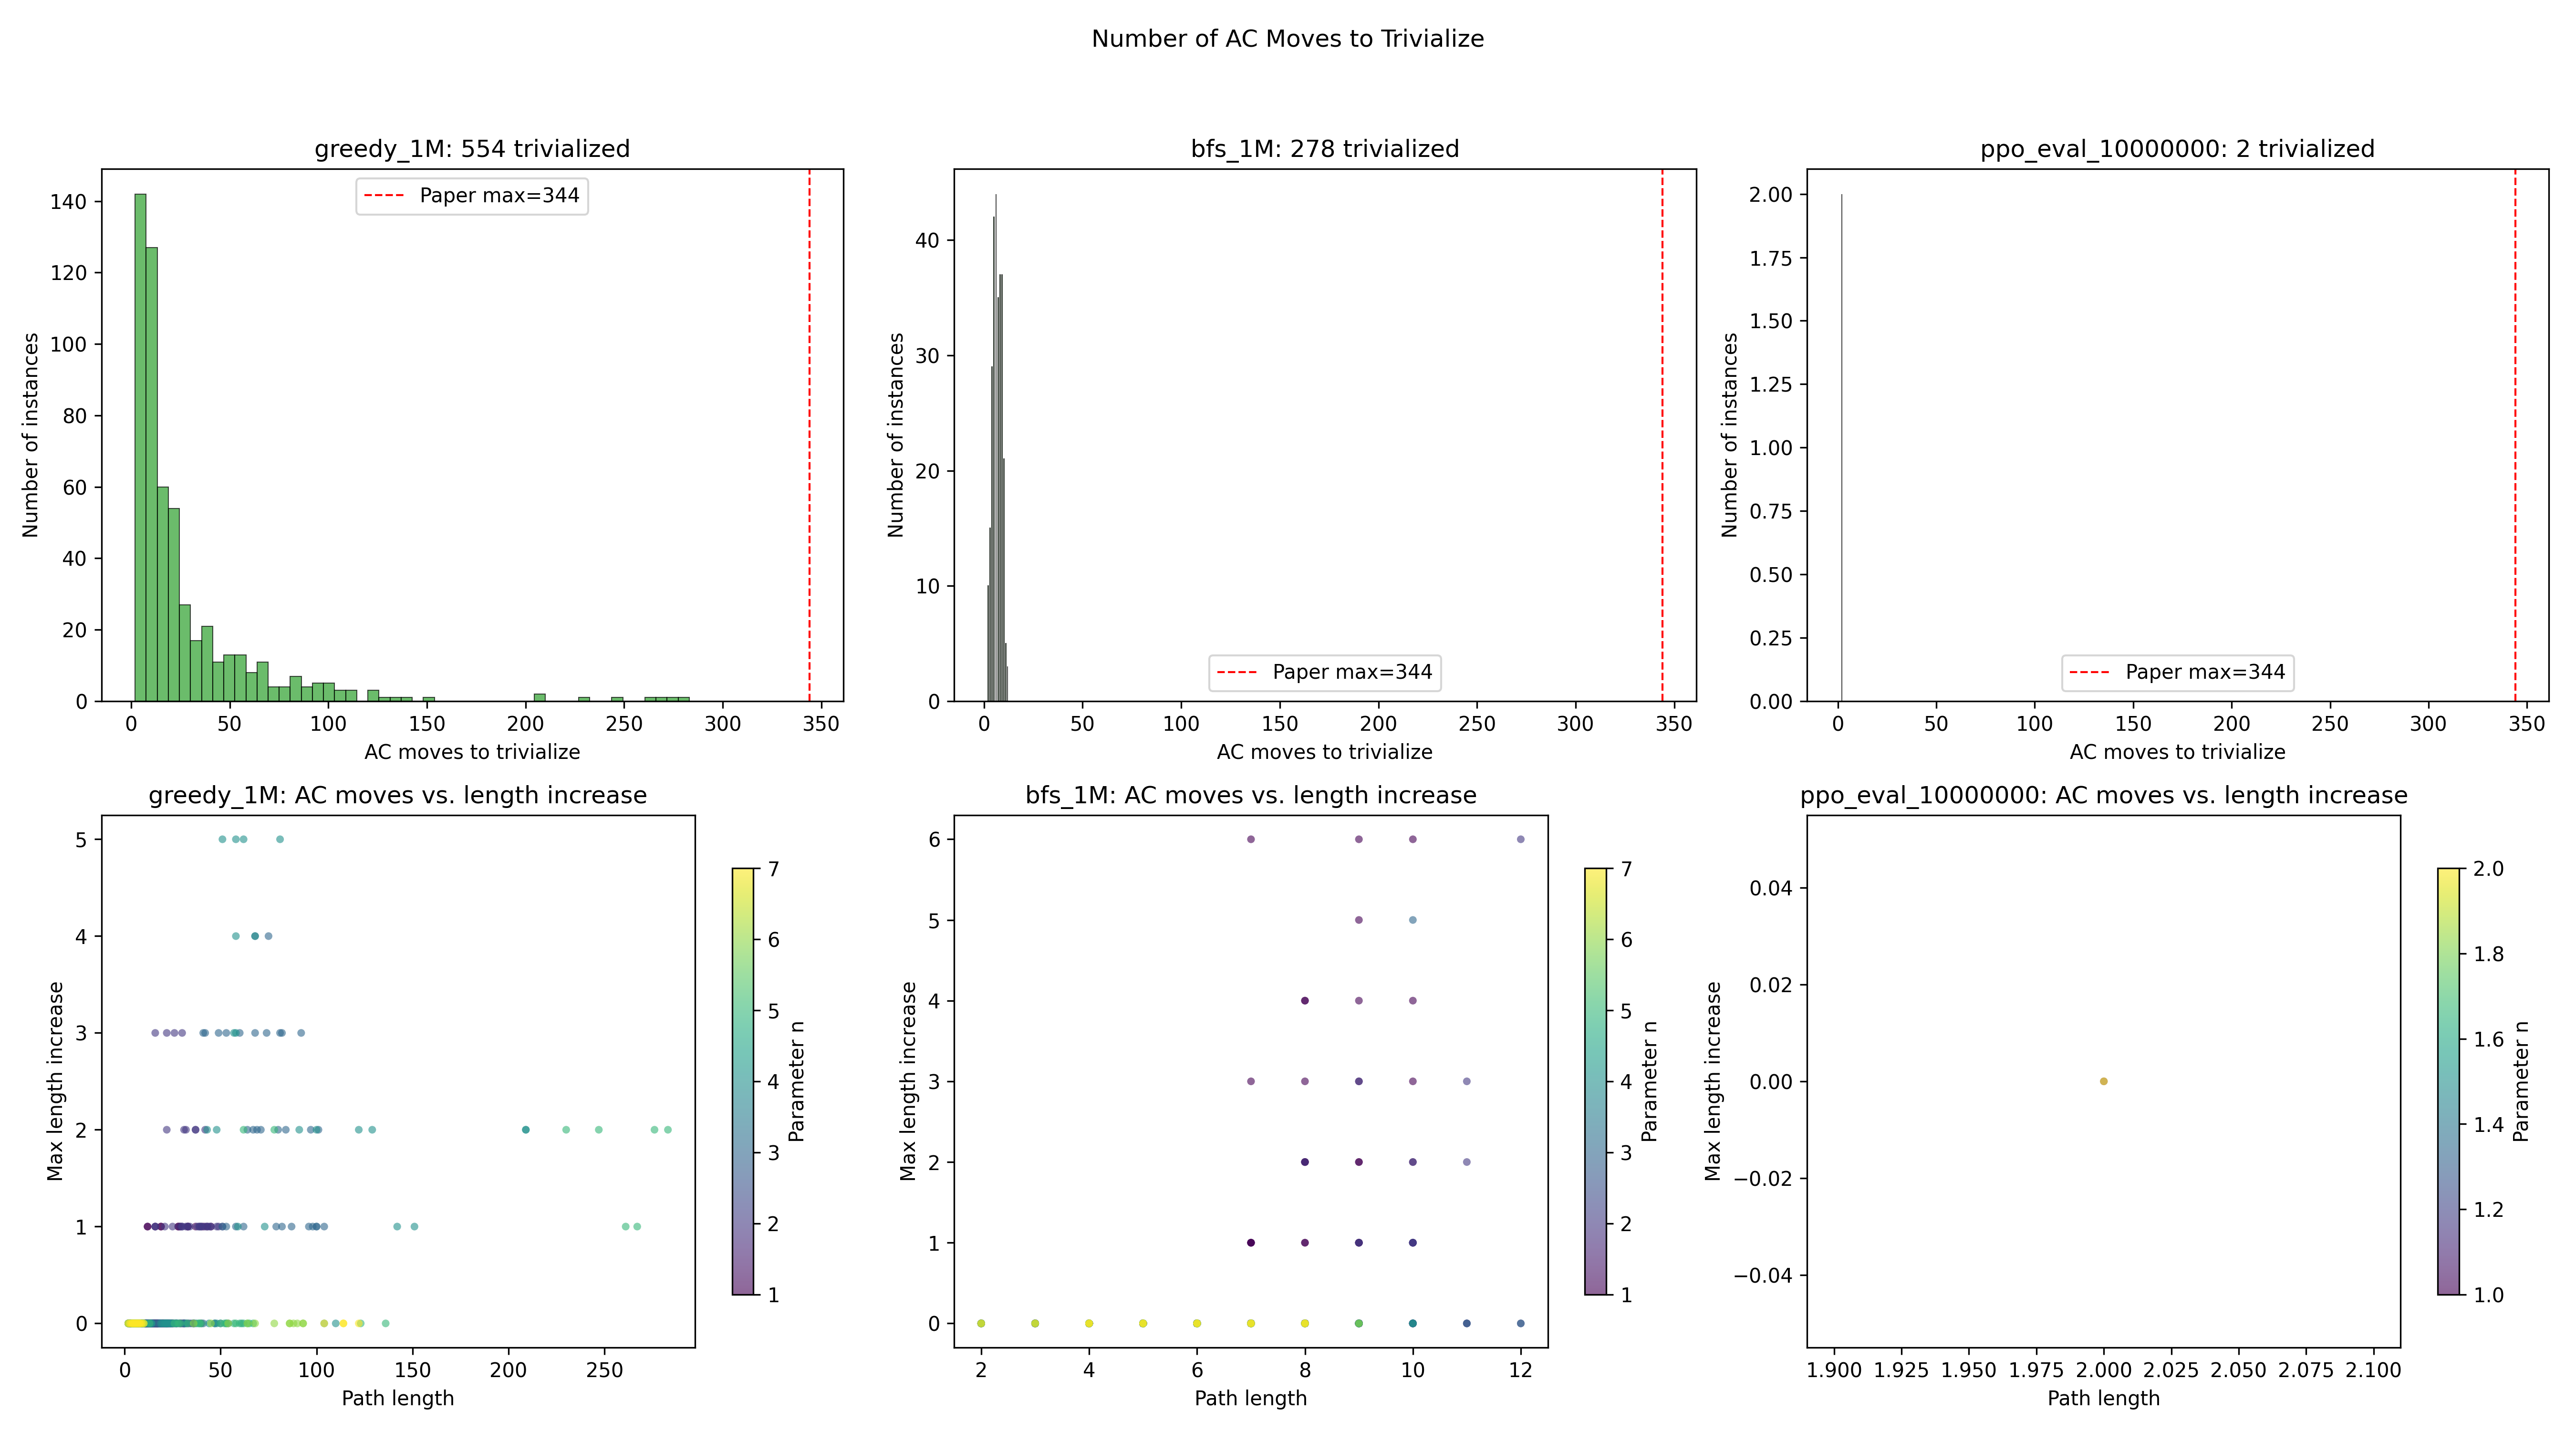
\includegraphics[width=0.65\textwidth]{figures/ac_path_steps_to_trivialization.png}
\caption{Distribution of path lengths (number of AC moves) for solved instances.}
\label{fig:path-lengths}
\end{figure}

% ══════════════════════════════════════════════════════════════════════════════
\section{PPO Reproduction}\label{sec:ppo}
% ══════════════════════════════════════════════════════════════════════════════

\subsection{Architecture}\label{sec:architecture}

The agent uses separate actor and critic networks, each a 2-layer
feed-forward MLP:

\begin{table}[h]
\centering
\caption{Actor--critic network architecture.}
\label{tab:architecture}
\begin{tabular}{lll}
  \toprule
  \textbf{Component} & \textbf{Architecture} & \textbf{Init} \\
  \midrule
  Actor  & $72 \to 512$ (Tanh) $\to 512$ (Tanh) $\to 12$  & Orthogonal ($\sqrt{2}$ hidden, $0.01$ output) \\
  Critic & $72 \to 512$ (Tanh) $\to 512$ (Tanh) $\to 1$   & Orthogonal ($\sqrt{2}$ hidden, $1.0$ output) \\
  \bottomrule
\end{tabular}
\end{table}

\begin{itemize}[nosep]
  \item \textbf{Input dimension:} $72 = 2 \times 36$ (two relators, each padded
    to \texttt{max\_relator\_length}).
  \item \textbf{Output:} 12 logits (one per AC move) for the actor; 1 scalar
    value for the critic.
  \item \textbf{Action selection:} $\mathrm{Categorical}(\text{logits})$ during
    training (stochastic); $\arg\max(\text{logits})$ during greedy evaluation
    (deterministic).
  \item \textbf{Weight initialisation:} Orthogonal with gain $\sqrt{2}$ for
    hidden layers, $0.01$ for the actor output layer (near-uniform initial
    policy), and $1.0$ for the critic output layer.
\end{itemize}

\paragraph{Source code.}
\texttt{ac\_solver/agents/ppo\_agent.py}.

% ──────────────────────────────────────────────────────────────────────────────
\subsection{Hyperparameters}\label{sec:hyperparams}

\begin{table}[h]
\centering
\caption{PPO hyperparameters: paper vs.\ our Mac reproduction.}
\label{tab:hyperparams}
\small
\begin{tabular}{lrrl}
  \toprule
  \textbf{Parameter} & \textbf{Paper} & \textbf{Mac Repro} & \textbf{Notes} \\
  \midrule
  \texttt{total\_timesteps}    & $10^8$  & $10^8$  & Same \\
  \texttt{num\_envs}           & 28      & 8       & Hardware constraint \\
  \texttt{num\_steps}          & 200     & 200     & Same (episode horizon) \\
  \texttt{batch\_size}         & 5{,}600 & 1{,}600 & $= \texttt{num\_envs} \times \texttt{num\_steps}$ \\
  \texttt{minibatch\_size}     & 1{,}400 & 400     & $= \texttt{batch\_size} / 4$ \\
  \texttt{num\_minibatches}    & 4       & 4       & Same \\
  \texttt{update\_epochs}      & 1       & 1       & Single pass per batch \\
  \texttt{learning\_rate}      & \multicolumn{2}{c}{$10^{-4} \to 0$ (linear)} & Same schedule \\
  $\gamma$                     & 0.999   & 0.999   & Discount factor \\
  $\lambda_{\text{GAE}}$       & 0.95    & 0.95    & GAE parameter \\
  $\epsilon_{\text{clip}}$     & 0.2     & 0.2     & PPO clip coefficient \\
  $c_{\text{ent}}$             & 0.01    & 0.01    & Entropy bonus \\
  $c_{\text{vf}}$              & 0.5     & 0.5     & Value loss coefficient \\
  \texttt{max\_grad\_norm}     & 0.5     & 0.5     & Gradient clipping \\
  $\mathrm{KL}_{\text{target}}$& 0.01   & 0.01    & Early stop threshold \\
  \texttt{repeat\_solved\_prob}& 0.25    & 0.25    & Curriculum revisit prob \\
  \midrule
  \textbf{PPO updates}         & 17{,}857 & 62{,}500 & $= \texttt{total\_timesteps} / \texttt{batch\_size}$ \\
  \bottomrule
\end{tabular}
\end{table}

The Mac run gets $3.5\times$ more PPO updates, but each with a $3.5\times$
smaller (and noisier) batch.

% ──────────────────────────────────────────────────────────────────────────────
\subsection{Reward Pipeline}\label{sec:reward}

The reward undergoes three transformations before reaching the PPO update:

\begin{enumerate}[nosep]
  \item \textbf{Raw reward} (from \texttt{ACEnv}):
    \begin{itemize}[nosep]
      \item Success: $+14{,}400$ ($ = \text{horizon} \times \texttt{max\_relator\_length} \times 2 = 200 \times 36 \times 2$)
      \item Per-step: $-\sum(\text{lengths})$ (typically $-5$ to $-70$)
    \end{itemize}

  \item \textbf{Reward clipping} to $[-10, 1000]$:
    \begin{itemize}[nosep]
      \item Success: $+14{,}400 \to +1{,}000$ \quad (\textbf{93\% of signal discarded})
      \item Per-step: $\max(-10, -\sum(\text{lengths}))$
    \end{itemize}

  \item \textbf{Division by \texttt{max\_reward}} ($= 14{,}400$):
    \begin{itemize}[nosep]
      \item Success: $+1{,}000 / 14{,}400 = +0.069$
      \item Per-step: $-10 / 14{,}400 = -0.00069$
    \end{itemize}
\end{enumerate}

\noindent
The net effect is a \textbf{$200\times$ attenuation} of the success signal.
This is the most significant concern with the current setup (see
Section~\ref{sec:diagnosis}).

% ──────────────────────────────────────────────────────────────────────────────
\subsection{Curriculum}\label{sec:curriculum}

\begin{itemize}[nosep]
  \item \textbf{Round~1:} Cycle through all 1190 presentations in order, one per
    episode reset.
  \item \textbf{Round~2+:} With probability $0.25$, revisit a solved
    presentation; otherwise pick an unsolved one.
  \item All 8 parallel environments independently track their position.
\end{itemize}

% ──────────────────────────────────────────────────────────────────────────────
\subsection{Training Execution}\label{sec:training-exec}

Training ran in two phases due to a session interruption:

\begin{table}[h]
\centering
\caption{Training execution phases.}
\label{tab:training-phases}
\begin{tabular}{lrrl}
  \toprule
  \textbf{Phase} & \textbf{Steps} & \textbf{Updates} & \textbf{Duration} \\
  \midrule
  Initial  & $0 \to 38.8\text{M}$   & $1 \to 24{,}285$       & $\sim$24 hours \\
  Resumed  & $38.7\text{M} \to 100\text{M}$ & $24{,}201 \to 62{,}500$ & $\sim$36 hours \\
  \midrule
  \textbf{Total} & $10^8$ & $62{,}500$ & $\sim$60 hours \\
  \bottomrule
\end{tabular}
\end{table}

Checkpoints were saved at \textbf{1M, 5M, 10M, 20M} (initial run) and
\textbf{50M, 100M} (resumed run).

% ──────────────────────────────────────────────────────────────────────────────
\subsection{Training Metrics}\label{sec:metrics}

\subsubsection{Metric Trajectory}

\begin{table}[h]
\centering
\caption{Key metrics at checkpoint steps.  ``Solved'' = cumulative presentations marked solved during training (stochastic).}
\label{tab:metric-trajectory}
\small
\begin{tabular}{rrrrrrr}
  \toprule
  \textbf{Step} & \textbf{Entropy} & \textbf{Logit Gap} & \textbf{Top-1 Prob} & \textbf{Expl.\ Var} & \textbf{Clip Frac} & \textbf{Solved} \\
  \midrule
  1{,}600 (start)  & 2.485 & 0.003 & 0.084 & $-0.920$ & 0.0 & 0/1190 \\
  1{,}000{,}000    & 2.483 & 0.035 & 0.093 & $-2.062$ & 0.0 & 116/1190 \\
  5{,}000{,}000    & 2.454 & 0.172 & 0.130 & $-1.332$ & 0.0 & 843/1190 \\
  10{,}000{,}000   & 1.919 & 1.162 & 0.397 & $+0.397$ & 0.0 & 1190/1190 \\
  20{,}000{,}000   & 1.363 & 1.667 & 0.591 & $+0.510$ & 0.0 & 1190/1190 \\
  50{,}000{,}000   & $\sim$1.2  & $\sim$1.4  & $\sim$0.58  & $\sim$0.6  & 0.0 & 1190/1190 \\
  100{,}000{,}000  & 1.253 & 1.415 & 0.601 & $+0.656$ & 0.0 & 1190/1190 \\
  \bottomrule
\end{tabular}
\end{table}

\subsubsection{Phase-Averaged Metrics}

\begin{table}[h]
\centering
\caption{Phase-averaged training metrics.}
\label{tab:phase-avg}
\small
\begin{tabular}{lrrrrr}
  \toprule
  \textbf{Phase} & \textbf{Avg Entropy} & \textbf{Avg Top-1} & \textbf{Avg Expl.\ Var} & \textbf{Avg Noop} & \textbf{Train Solve Rate} \\
  \midrule
  0--1M   & 2.484 & 0.089 & $-1.832$ & 0.604 & 2.5\% \\
  1--5M   & 2.470 & 0.109 & $-1.834$ & 0.607 & 4.7\% \\
  5--10M  & 2.283 & 0.229 & $-0.559$ & 0.632 & 49.3\% \\
  10--20M & 1.664 & 0.482 & $+0.371$ & 0.674 & 88.0\% \\
  20--50M & 1.254 & 0.592 & $+0.690$ & 0.666 & 94.1\% \\
  50--100M & 1.235 & 0.594 & $+0.734$ & 0.656 & 94.5\% \\
  \bottomrule
\end{tabular}
\end{table}

\subsubsection{Evidence of Network Change}

Four independent metrics confirm the policy parameters changed significantly:
\begin{enumerate}[nosep]
  \item \textbf{Entropy:} $2.485 \to 1.253$.  A uniform policy over 12 actions
    has entropy $\ln(12) \approx 2.485$.  The final value indicates the policy
    concentrates probability mass on a subset of actions.
  \item \textbf{Top-1 probability:} $8.4\% \to 60.1\%$.  A uniform policy
    assigns $1/12 \approx 8.3\%$ to each action.
  \item \textbf{Logit gap:} $0.003 \to 1.415$.  The actor developed distinct
    preferences between actions.
  \item \textbf{Explained variance:} $-0.92 \to +0.66$.  The critic learned to
    predict which states lead to success.
\end{enumerate}

\subsubsection{Why \texttt{clipfrac} = 0 Throughout}

With \texttt{update\_epochs}~$= 1$, each batch is processed in a single pass
through 4~minibatches.  The first minibatch sees an \emph{unchanged} network
(ratio~$= 1.0$ exactly).  Subsequent minibatches see a network shifted by 1--3
gradient steps, but with:
\begin{itemize}[nosep]
  \item normalised advantages of std~$\approx 0.03$,
  \item gradient norm clipped to 0.5,
  \item learning rate $\le 10^{-4}$,
\end{itemize}
the policy ratio stays well within $[0.8, 1.2]$.  This is \emph{expected
behaviour}, not a bug.  Over 62{,}500 updates, these small changes accumulate
into the large entropy reduction observed.

\subsubsection{Action Distribution Shift}

\begin{figure}[ht]
\centering
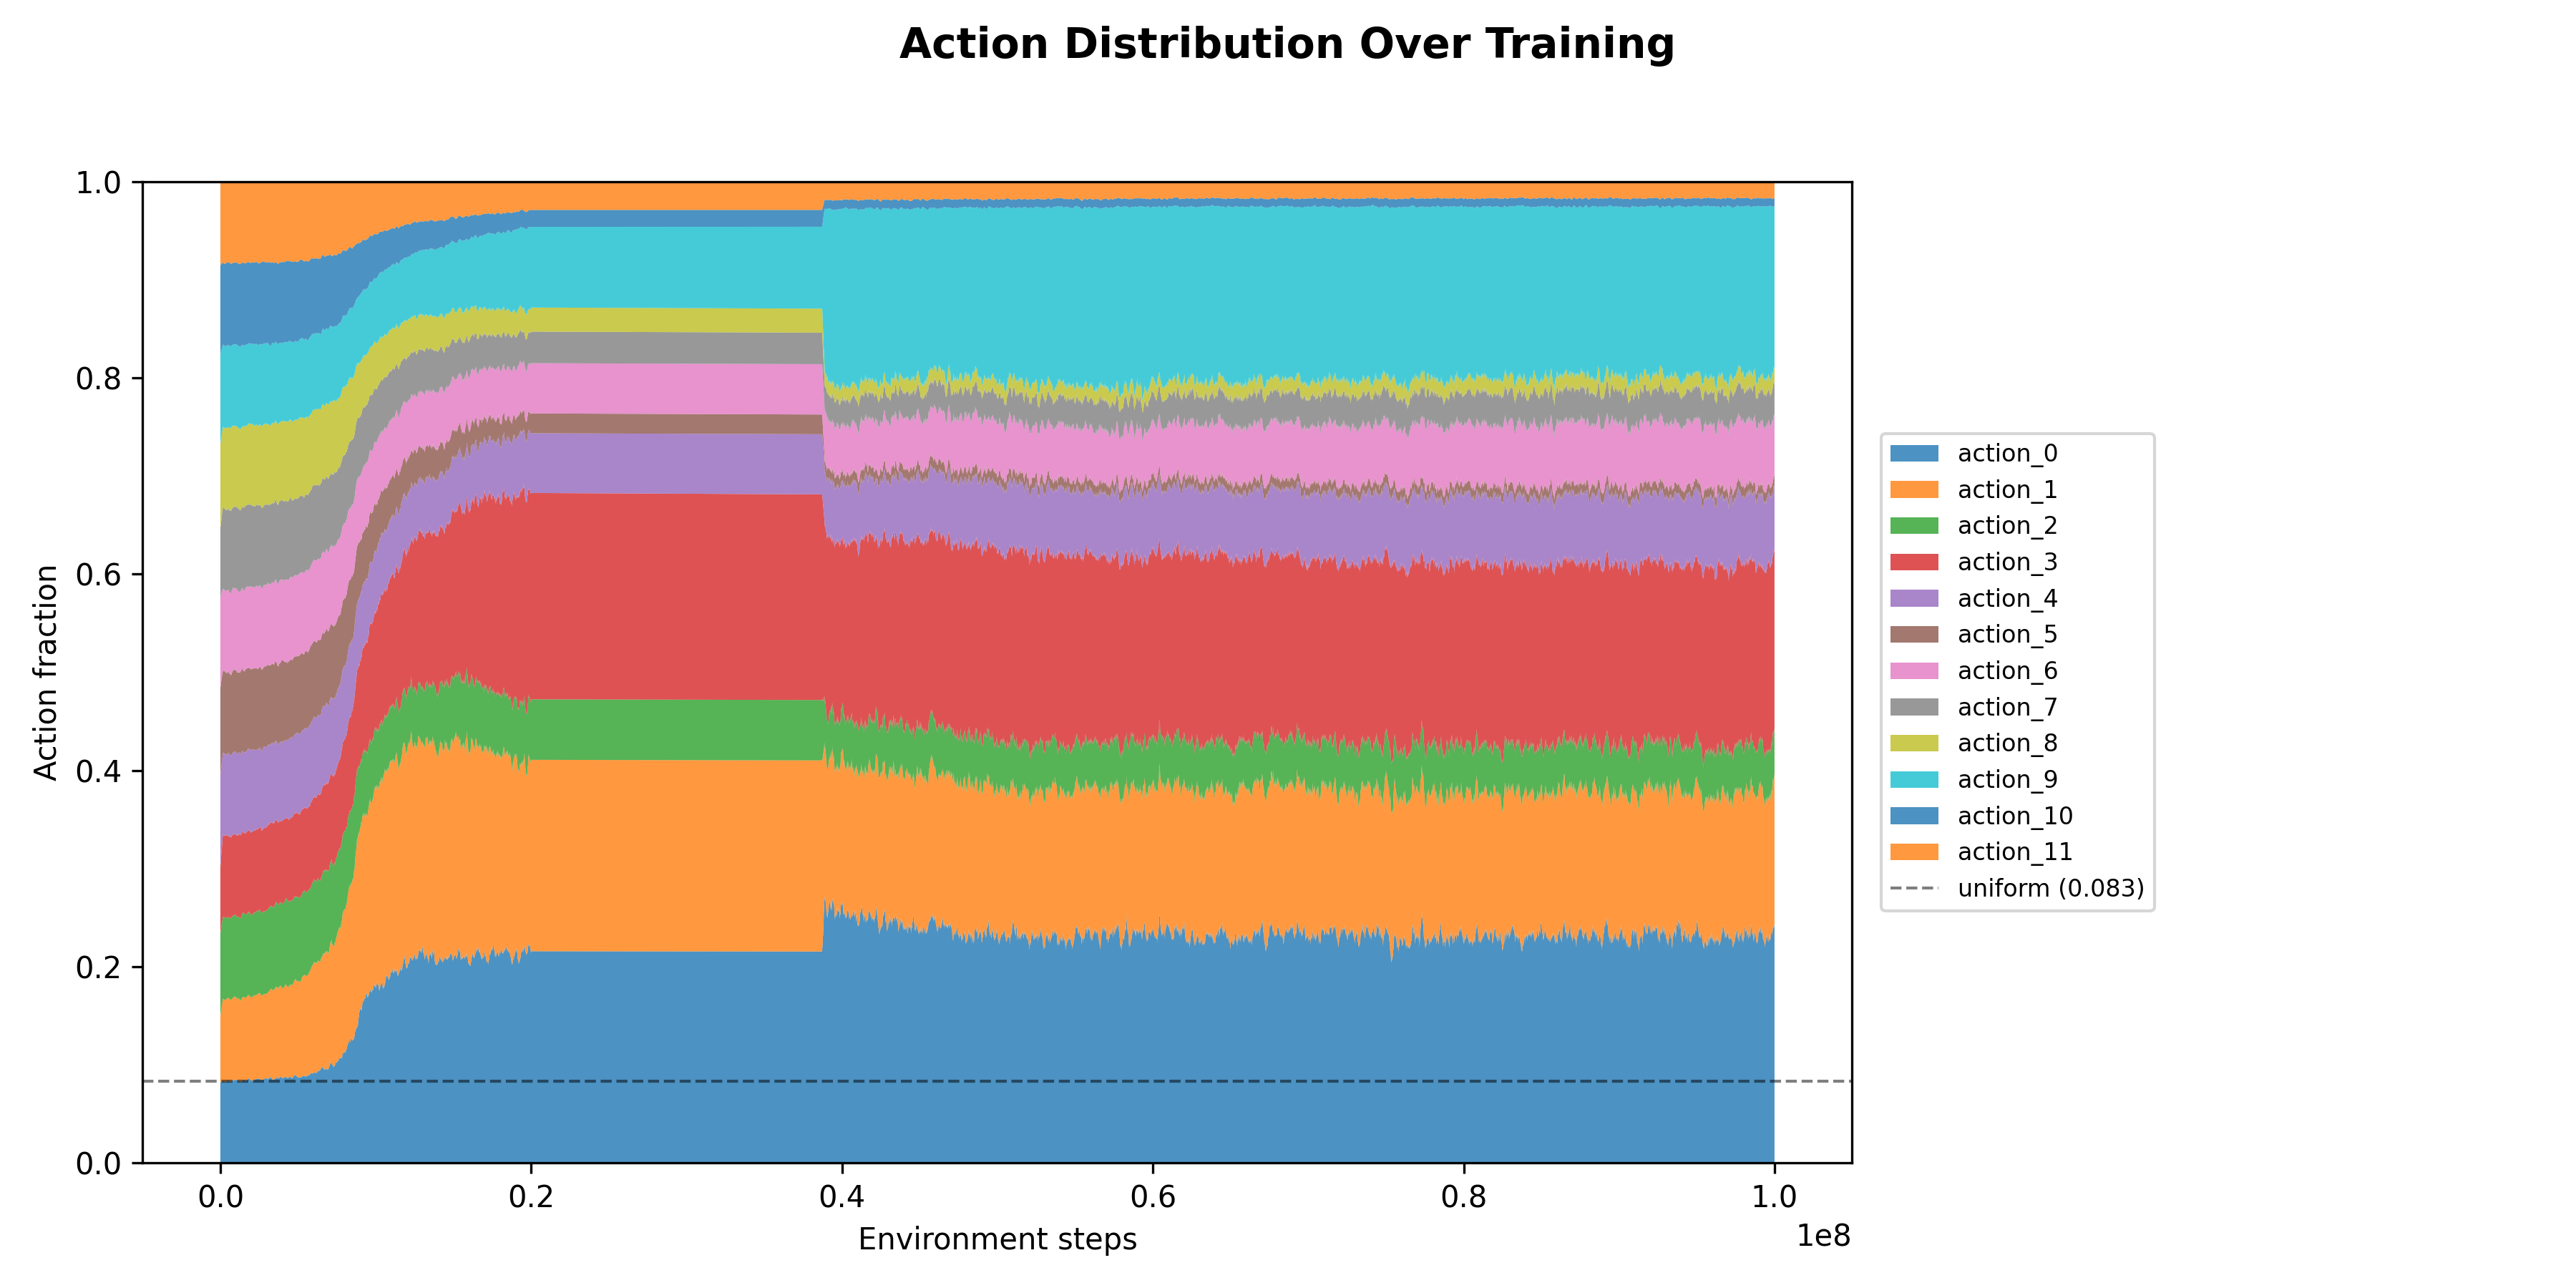
\includegraphics[width=0.75\textwidth]{figures/action_distribution.png}
\caption{Action frequency distribution over training.  The policy shifts from
uniform ($\sim$8.3\% each) to concentrated, favouring concatenation moves
(actions 0, 1, 3) over conjugations.}
\label{fig:action-dist}
\end{figure}

The policy learned to favour concatenation moves (actions~0--3), which are the
primary mechanism for reducing relator lengths.  Certain conjugations
(actions~5, 8, 10, 11) are used very rarely ($<3\%$ each).

\subsubsection{Training Curves}

\begin{figure}[ht]
\centering
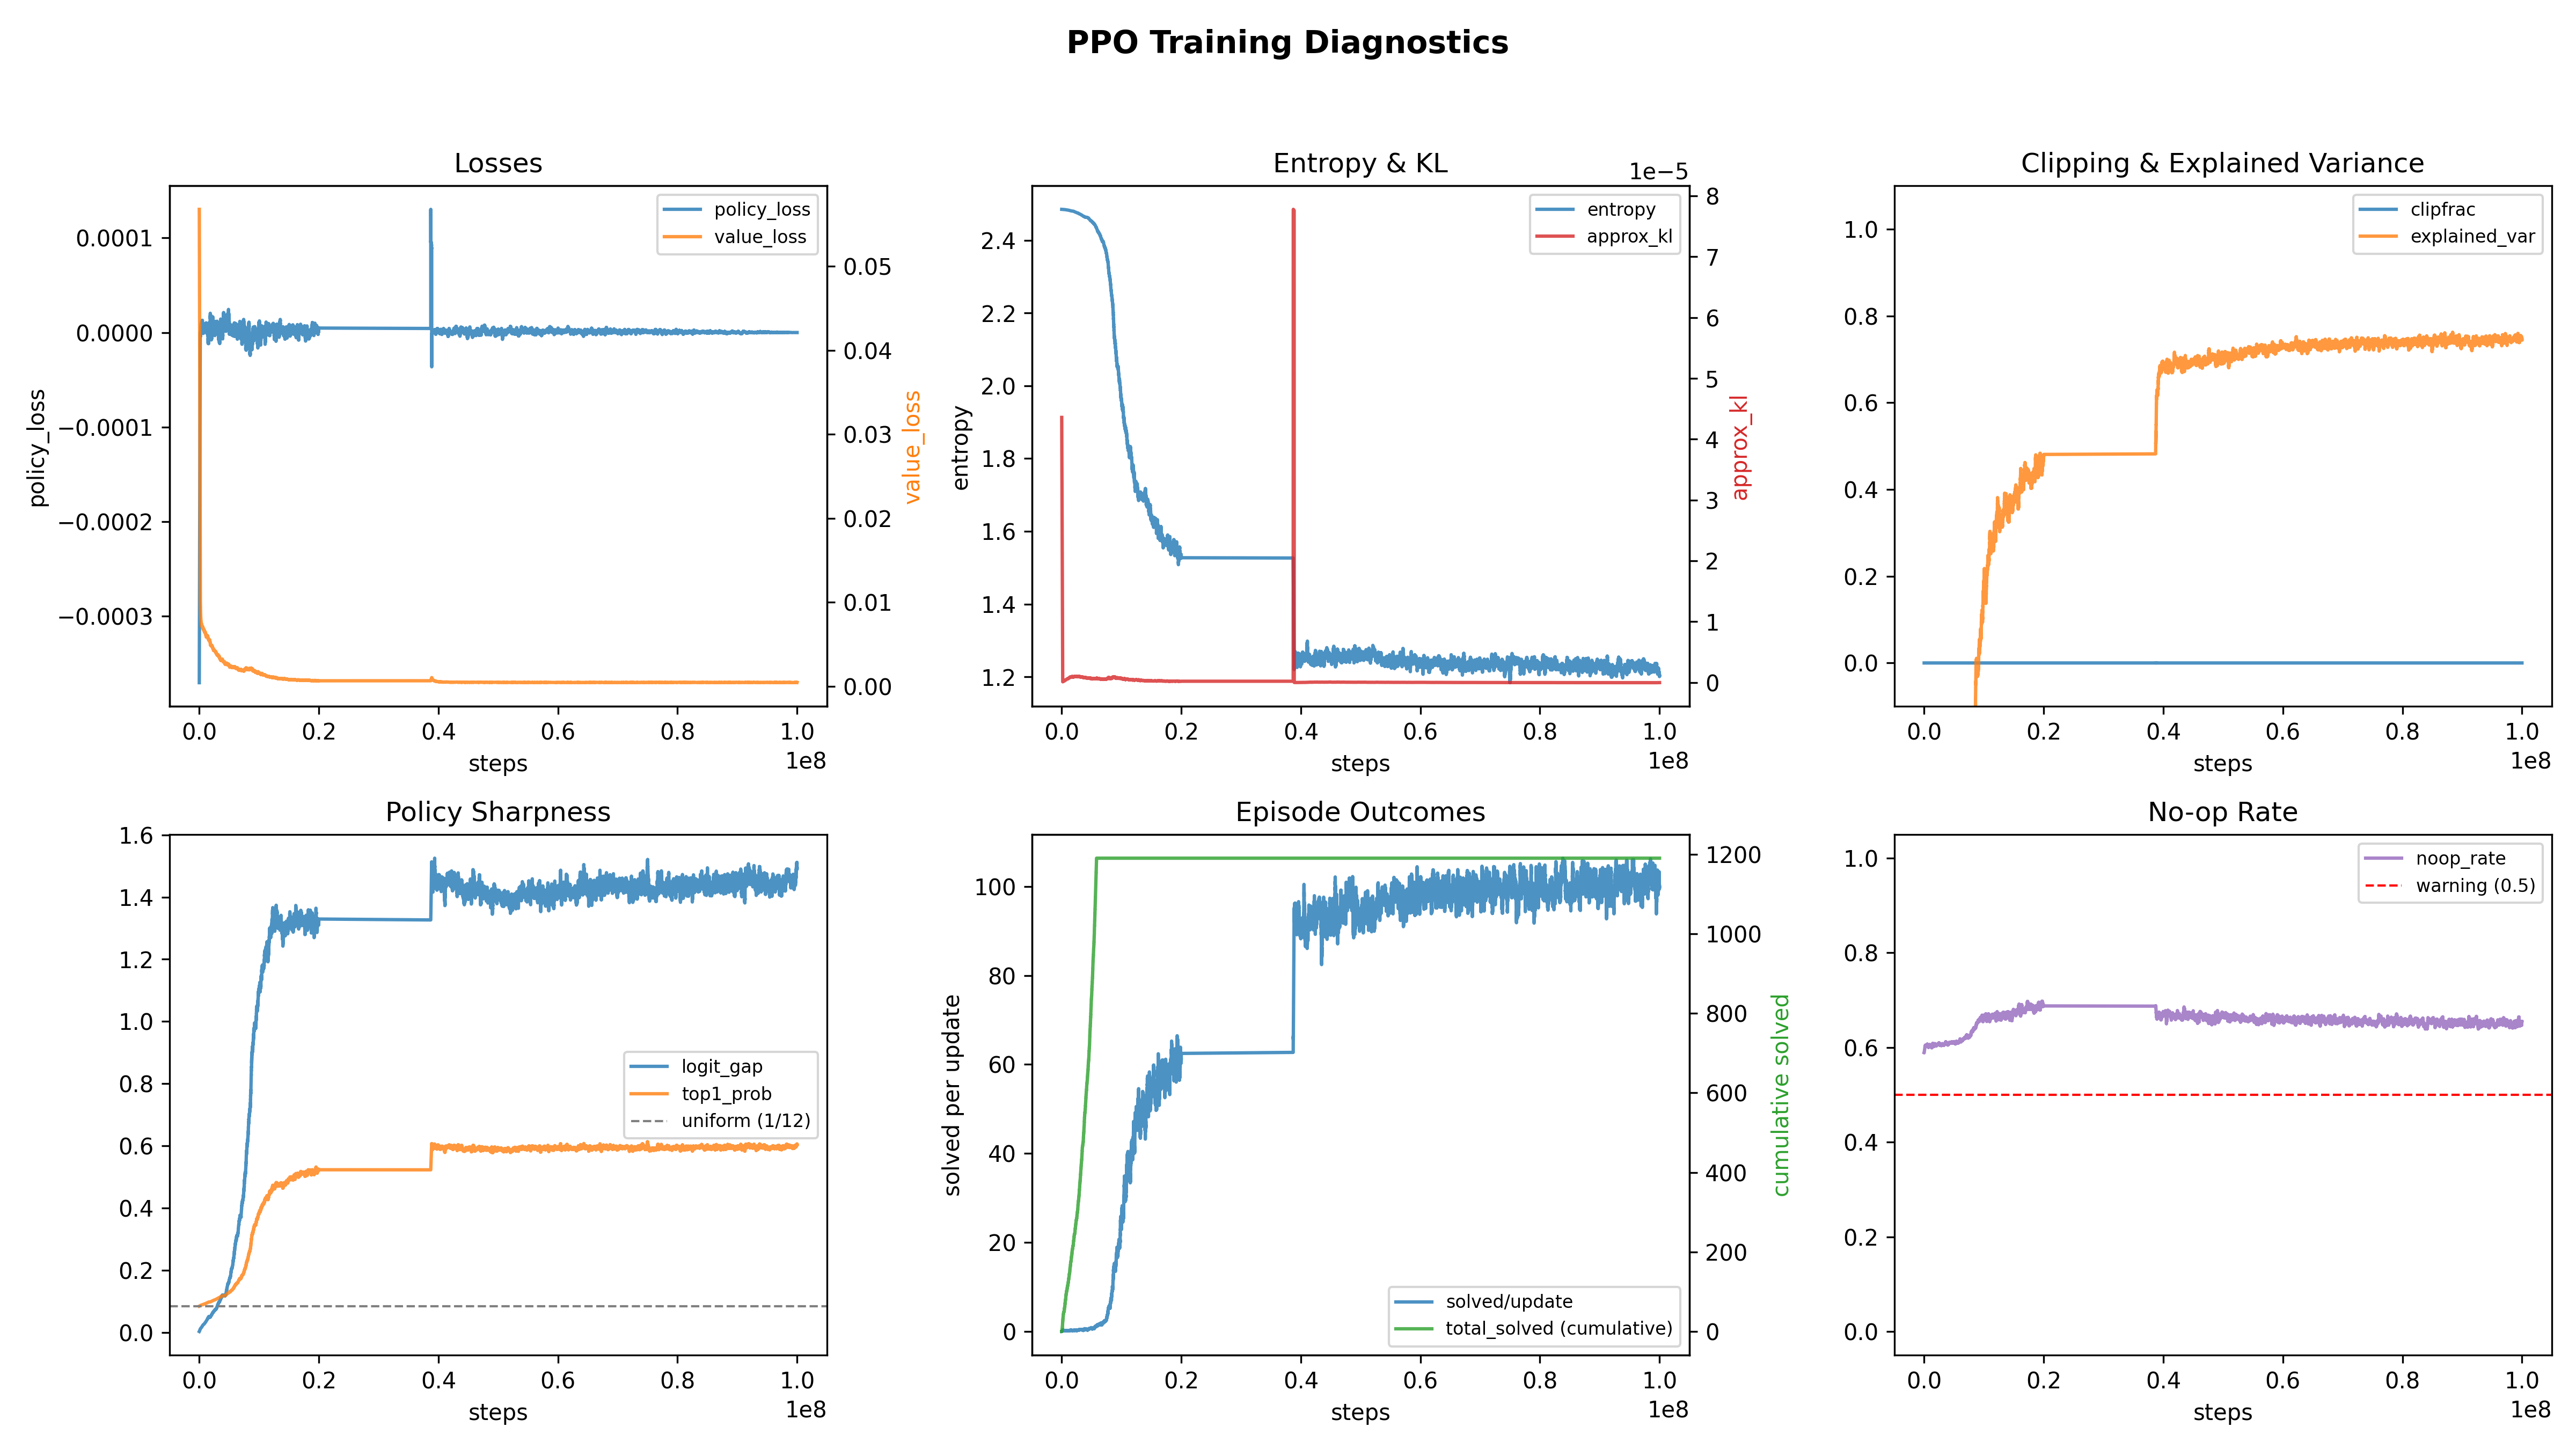
\includegraphics[width=\textwidth]{figures/training_diagnostics.png}
\caption{Training diagnostics (2$\times$3 grid).
  \textbf{Top:} losses, entropy/KL, clipping/explained variance.
  \textbf{Bottom:} policy sharpness (logit gap, top-1 prob), episode outcomes,
  noop rate.}
\label{fig:training-curves}
\end{figure}

% ──────────────────────────────────────────────────────────────────────────────
\subsection{Evaluation Results}\label{sec:eval}

We evaluated 6~checkpoints across 3 modes on the full 1190-instance dataset
with horizon = 200:

\begin{itemize}[nosep]
  \item \textbf{Greedy (deterministic):} $\text{action} = \arg\max(\text{logits})$
  \item \textbf{Stochastic ($\times 1$):} $\text{action} \sim \mathrm{Categorical}(\text{logits})$
  \item \textbf{Stochastic ($\times 5$, best-of-5):} 5 independent rollouts, report best
\end{itemize}

\begin{table}[h]
\centering
\caption{PPO evaluation results (solved out of 1190 instances).}
\label{tab:ppo-eval}
\begin{tabular}{lrrr}
  \toprule
  \textbf{Checkpoint} & \textbf{Greedy (det)} & \textbf{Stoch $\times$1} & \textbf{Stoch $\times$5} \\
  \midrule
  1M   & 0 (0.0\%)  & 2 (0.2\%)   & 7 (0.6\%)   \\
  5M   & 5 (0.4\%)  & 6 (0.5\%)   & 15 (1.3\%)  \\
  10M  & 7 (0.6\%)  & 12 (1.0\%)  & 30 (2.5\%)  \\
  20M  & 7 (0.6\%)  & 10 (0.8\%)  & 30 (2.5\%)  \\
  \textbf{50M}  & \textbf{6 (0.5\%)}  & \textbf{16 (1.3\%)}  & \textbf{32 (2.7\%)} \\
  100M & 6 (0.5\%)  & 13 (1.1\%)  & 29 (2.4\%)  \\
  \bottomrule
\end{tabular}
\end{table}

\textbf{Peak performance is at 50M steps}, not 100M---the linear LR$\to$0
schedule degraded the policy in the second half of training.

\subsubsection{Comparison with Classical Baselines}

\begin{table}[h]
\centering
\caption{PPO vs.\ classical baselines.}
\label{tab:ppo-vs-classical}
\begin{tabular}{lrr}
  \toprule
  \textbf{Algorithm} & \textbf{Solved} & \textbf{Solve Rate} \\
  \midrule
  Greedy search ($10^6$ nodes)           & 554 / 1190 & 46.6\% \\
  BFS ($10^6$ nodes)                     & 278 / 1190 & 23.4\% \\
  PPO 50M greedy (best det)              & 6 / 1190   & 0.5\%  \\
  PPO 50M best-of-5 stoch (best overall) & 32 / 1190  & 2.7\%  \\
  \bottomrule
\end{tabular}
\end{table}

Classical greedy search (a simple heuristic with no learning) solves
\textbf{$17\times$ more} presentations than the best PPO configuration.

\subsubsection{PPO vs.\ Random Baseline}

To determine whether PPO learned anything useful, we compare the best PPO
checkpoint (50M best-of-5) against a near-random policy (1M best-of-5):

\begin{table}[h]
\centering
\caption{PPO vs.\ near-random policy.}
\label{tab:ppo-vs-random}
\begin{tabular}{lrl}
  \toprule
  \textbf{Policy} & \textbf{Best-of-5 Solved} & \textbf{Interpretation} \\
  \midrule
  Near-random (1M)   & 7 / 1190 (0.6\%)  & Random walk baseline \\
  PPO 50M            & 32 / 1190 (2.7\%) & $4.6\times$ improvement \\
  Overlap            & 4                  & Solved by both \\
  PPO-only           & 28                 & Genuine learning \\
  Random-only        & 3                  & Noise \\
  \bottomrule
\end{tabular}
\end{table}

The PPO policy is \textbf{significantly better than random} ($4.6\times$),
confirming genuine learning.  However, it solves only the easiest instances
(short initial lengths, low $n$).

\paragraph{How to reproduce PPO evaluation.}
\begin{lstlisting}[language=bash]
# Deterministic evaluation on full dataset
python -m ac_solver.agents.evaluate \
    --checkpoint out/<run_dir>/ckpt_50000000.pt \
    --horizon 200 --full \
    --output results/ppo_50M_det.csv

# Stochastic best-of-5
python -m ac_solver.agents.evaluate \
    --checkpoint out/<run_dir>/ckpt_50000000.pt \
    --horizon 200 --full --stochastic --num-rollouts 5 \
    --eval-seed 42 --output results/ppo_50M_sto5.csv
\end{lstlisting}

% ══════════════════════════════════════════════════════════════════════════════
\section{Diagnosis and Recommendations}\label{sec:diagnosis}
% ══════════════════════════════════════════════════════════════════════════════

\subsection{Why PPO Underperformed}

\begin{enumerate}
  \item \textbf{Catastrophic reward attenuation.}  The success reward
    ($+14{,}400$) is clipped to $+1{,}000$ then divided by $14{,}400$, yielding
    a final signal of $+0.069$---a $200\times$ reduction.  The policy gradient
    is dominated by noise for most updates.

  \item \textbf{Insufficient data reuse.}  With \texttt{update\_epochs}~$= 1$,
    each batch of experience is used exactly once.  Standard PPO uses 3--10
    epochs.

  \item \textbf{Batch size too small.}  The $1{,}600$-sample batch (vs.\
    paper's $5{,}600$) yields $3.5\times$ noisier gradient estimates per update.

  \item \textbf{LR$\to$0 degradation.}  Linear annealing to zero means the
    last $\sim$10\% of training has negligible learning.  The 50M checkpoint
    outperforms the 100M checkpoint.

  \item \textbf{Misleading training metrics.}  The 100\% training solve rate
    (by 10M steps) reflects stochastic exploration during 200-step rollouts,
    not learned policy quality.  At 2.5\% solve rate, even a near-random policy
    ``solves'' many presentations via random walks.

  \item \textbf{High noop rate ($\sim$69\%).}  Two-thirds of actions produce no
    state change, wasting the action budget.
\end{enumerate}

\subsection{Recommended Next Steps (Ranked by Expected Impact)}

\begin{enumerate}
  \item \textbf{Fix reward scaling.}  Either remove the \texttt{clip\_rewards}
    step (letting the full $+14{,}400$ signal through) or use running
    normalisation via \texttt{gym.wrappers.NormalizeReward} instead of the fixed
    division by \texttt{max\_reward}.

  \item \textbf{Increase \texttt{update\_epochs} to 4.}  Extract $4\times$ more
    learning per batch.  The \texttt{target\_kl}~$= 0.01$ early stop prevents
    overfitting.

  \item \textbf{Increase \texttt{num\_envs}} to 16 or 28 if hardware permits,
    improving gradient quality and presentation diversity per batch.

  \item \textbf{Use cosine annealing with \texttt{min\_lr\_frac}~$= 0.1$.}
    Maintain a learning rate floor of $10^{-5}$ instead of decaying to zero.

  \item \textbf{Add action masking.}  Prevent the agent from selecting moves
    that would exceed \texttt{max\_relator\_length}, reducing the effective
    action space and noop rate.

  \item \textbf{Monitor greedy eval during training.}  Add periodic greedy
    evaluation (e.g.\ every $10^6$ steps on a small subset) as the ground-truth
    metric, since training solve rate is misleading.
\end{enumerate}

% ══════════════════════════════════════════════════════════════════════════════
\section{Conclusions}\label{sec:conclusions}
% ══════════════════════════════════════════════════════════════════════════════

\paragraph{Was the training code correct?}
Yes, mechanically.  The PPO implementation is standard and bug-free.  All
hyperparameters match or closely approximate the paper's configuration
(adjusted for hardware).  The persistent \texttt{clipfrac}~$= 0$ is a
consequence of conservative hyperparameters (\texttt{update\_epochs}~$= 1$,
small reward signal), not a bug.

\paragraph{Did the policy learn?}
Weakly.  The best configuration (50M, best-of-5 stochastic) solves 32/1190
instances (2.7\%)---a $4.6\times$ improvement over a near-random baseline
(7/1190), with 28~instances solved exclusively by the trained policy.  However,
this is $17\times$ worse than classical greedy search (554/1190).

\paragraph{Classical search remains far superior.}
Greedy search, a simple heuristic requiring no training, solves 46.6\% of the
dataset.  BFS, which guarantees optimal path length, solves 23.4\%.  Both vastly
outperform the PPO agent, suggesting that the current RL formulation does not
effectively capture the combinatorial structure of the Andrews--Curtis problem.

% ══════════════════════════════════════════════════════════════════════════════
\appendix
\section{Reproduction Commands}\label{sec:commands}
% ══════════════════════════════════════════════════════════════════════════════

\subsection{Classical Search}

\begin{lstlisting}[language=bash]
# Greedy search: full dataset, 1M node budget
python -m ac_solver.search.miller_schupp.evaluate \
    --search-fn greedy --max-nodes 1000000 \
    --workers 4 --full --output results/greedy_1M.csv

# BFS: full dataset, 1M node budget
python -m ac_solver.search.miller_schupp.evaluate \
    --search-fn bfs --max-nodes 1000000 \
    --workers 4 --full --output results/bfs_1M.csv

# Resume an interrupted run
python -m ac_solver.search.miller_schupp.evaluate \
    --search-fn greedy --max-nodes 1000000 \
    --workers 8 --full --output results/greedy_1M.csv --resume

# Run on a single presentation
python ac_solver/search/greedy.py --preset AK2 --max-nodes 100000

# Run BFS on a specific presentation string
python ac_solver/search/breadth_first.py \
    --presentation "1,1,-2,-2,-2,0,0,1,2,1,-2,-1,-2,0" \
    --max-nodes 500000
\end{lstlisting}

\subsection{PPO Training}

\begin{lstlisting}[language=bash]
# Train with paper-faithful Mac preset (100M steps, 8 envs)
python -m ac_solver.agents.ppo \
    --preset paper_faithful_mac \
    --seed 1 \
    --exp-name paper_faithful_mac_s1

# Resume from checkpoint
python -m ac_solver.agents.ppo \
    --preset paper_faithful_mac \
    --seed 1 \
    --exp-name paper_faithful_mac_s1_resumed \
    --resume --checkpoint-dir out/<previous_run_dir>
\end{lstlisting}

\subsection{PPO Evaluation}

\begin{lstlisting}[language=bash]
# Deterministic (greedy) evaluation
python -m ac_solver.agents.evaluate \
    --checkpoint out/<run_dir>/ckpt_50000000.pt \
    --horizon 200 --full \
    --output results/ppo_50M_det.csv

# Stochastic single rollout
python -m ac_solver.agents.evaluate \
    --checkpoint out/<run_dir>/ckpt_50000000.pt \
    --horizon 200 --full --stochastic \
    --output results/ppo_50M_sto.csv

# Best-of-5 stochastic
python -m ac_solver.agents.evaluate \
    --checkpoint out/<run_dir>/ckpt_50000000.pt \
    --horizon 200 --full --stochastic --num-rollouts 5 \
    --eval-seed 42 --output results/ppo_50M_sto5.csv

# Best-of-32 (high rollout count)
python -m ac_solver.agents.evaluate \
    --checkpoint out/<run_dir>/ckpt_100000000.pt \
    --horizon 200 --full --stochastic --num-rollouts 32 \
    --eval-seed 42 --output results/ppo_100M_sto32.csv
\end{lstlisting}

\subsection{Plotting}

\begin{lstlisting}[language=bash]
# Training curves from metrics CSV
python -m ac_solver.agents.plot_training_curves \
    --csv report/metrics_combined.csv --output-dir report/

# Classical search result figures
python -m ac_solver.search.miller_schupp.plot_results \
    --csvs results/greedy_1M.csv results/bfs_1M.csv \
    --output-dir results/figures/
\end{lstlisting}

% ──────────────────────────────────────────────────────────────────────────────
\section{CSV Output Schema}\label{sec:csv-schema}

\subsection{Classical Search CSV}

Each row corresponds to one presentation instance:

\begin{table}[h]
\centering
\small
\begin{tabular}{lp{8cm}}
  \toprule
  \textbf{Field} & \textbf{Description} \\
  \midrule
  \texttt{instance\_id}       & Integer index (0--1189) \\
  \texttt{n}                  & Miller--Schupp parameter $n$ \\
  \texttt{lenw}               & Word length $|w|$ \\
  \texttt{algorithm}          & \texttt{greedy} or \texttt{bfs} \\
  \texttt{max\_nodes}         & Node budget \\
  \texttt{solved}             & \texttt{True}/\texttt{False} \\
  \texttt{visited\_nodes}     & Unique states explored \\
  \texttt{path\_length}       & Number of AC moves in solution \\
  \texttt{initial\_total\_length} & Starting $|r_0| + |r_1|$ \\
  \texttt{max\_intermediate\_length} & Peak length during search \\
  \texttt{length\_increase}   & $\text{max\_intermediate} - \text{initial}$ \\
  \texttt{wallclock\_seconds} & Elapsed time \\
  \bottomrule
\end{tabular}
\end{table}

\subsection{PPO Evaluation CSV}

Same schema as classical search, with \texttt{algorithm} set to \texttt{ppo}
(deterministic) or \texttt{ppo\_stochastic} (sampling).

% ──────────────────────────────────────────────────────────────────────────────
\section{Checkpoint Inventory}\label{sec:checkpoints}

\begin{table}[h]
\centering
\small
\begin{tabular}{lrl}
  \toprule
  \textbf{File} & \textbf{Steps} & \textbf{Directory} \\
  \midrule
  \texttt{ckpt\_1000000.pt}    & 1M   & \texttt{out/paper\_faithful\_mac\_s1\_ppo-ffn-nodes\ldots f6f8985b\ldots} \\
  \texttt{ckpt\_5000000.pt}    & 5M   & (same) \\
  \texttt{ckpt\_10000000.pt}   & 10M  & (same) \\
  \texttt{ckpt\_20000000.pt}   & 20M  & (same) \\
  \texttt{ckpt\_50000000.pt}   & 50M  & \texttt{out/paper\_faithful\_mac\_s1\_resumed\ldots c3f0ba19\ldots} \\
  \texttt{ckpt\_100000000.pt}  & 100M & (same) \\
  \bottomrule
\end{tabular}
\end{table}

\end{document}
